\documentclass[8pt,xcolor=dvipsnames]{beamer}
\usepackage[latin1]{inputenc}

\usetheme[height=7mm]{Berlin}
\usecolortheme[named=Brown]{structure} 


\usepackage{time}       % date and time
\usepackage{graphicx}
\usepackage[T1]{fontenc}    % european characters
%\usepackage{courier}
\usepackage{animate}
\usepackage{multirow}
\usepackage{natbib}
\usepackage{amssymb,amsmath}  % use mathematical symbols
\usepackage{bookman}                  % use palatino as the default font
\setbeamercovered{transparent}
%\newcommand{figpath}{/Users/bhargavvaidya/MyProject/work/Leeds_Uni/SiOJets_New/PAPER/PFIGS}

\title[SiO Outflows]{Modeling SiO Emission from early outflows}
\subtitle{Extremely High Velocity Component [ EHV ]}
\author[Bhargav Vaidya]{\textcolor{blue}{Bhargav Vaidya}\inst{1} \and  Thomas
  Douglas\inst{1} \and Paola Caselli\inst{1}}\institute[Uni. Leeds]{\inst{1}School of Physics and
  Astronomy, University of Leeds, Leeds.}
\date[2013]{AG Annual Meeting 2013}
\titlegraphic{\vskip30pt \hskip215pt
\includegraphics[width=0.3\textwidth]{/Users/bhargavvaidya/MyProject/work/Leeds_Uni/SiOJets_New/PAPER/PFIGS/Leeds-logo.jpg}}

\begin{document}

\begin{frame}
\titlepage
\end{frame}

\begin{frame}
\frametitle{Outline}
\tableofcontents
\end{frame}

\section{Motivation}
\begin{frame}[t]
\frametitle{Motivation}
\small{
\begin{block}{EHV Emission}
\begin{itemize}
\item Observed for the first time in L1448 outflow (\alert{Bachiller
    1991})
\item Associated with primary jet (\alert{Santiago-Garcia, 2009}, {\it{IRAS 04166+2706}}). Observed in SiO, CO but no signatures in HCN or CS (\alert{Tafalla, 2010}).
\item How are they formed ? J-shocks or C-shocks ? Stationary 1D
  Models -- FAILS! (557 GHz \alert{Tafalla, 2013}) \textbf{NEED FOR A 2D MODEL!}
\end{itemize}
\end{block}
}
\vskip10pt
\begin{columns}[C]
\begin{column}{0.5\textwidth}
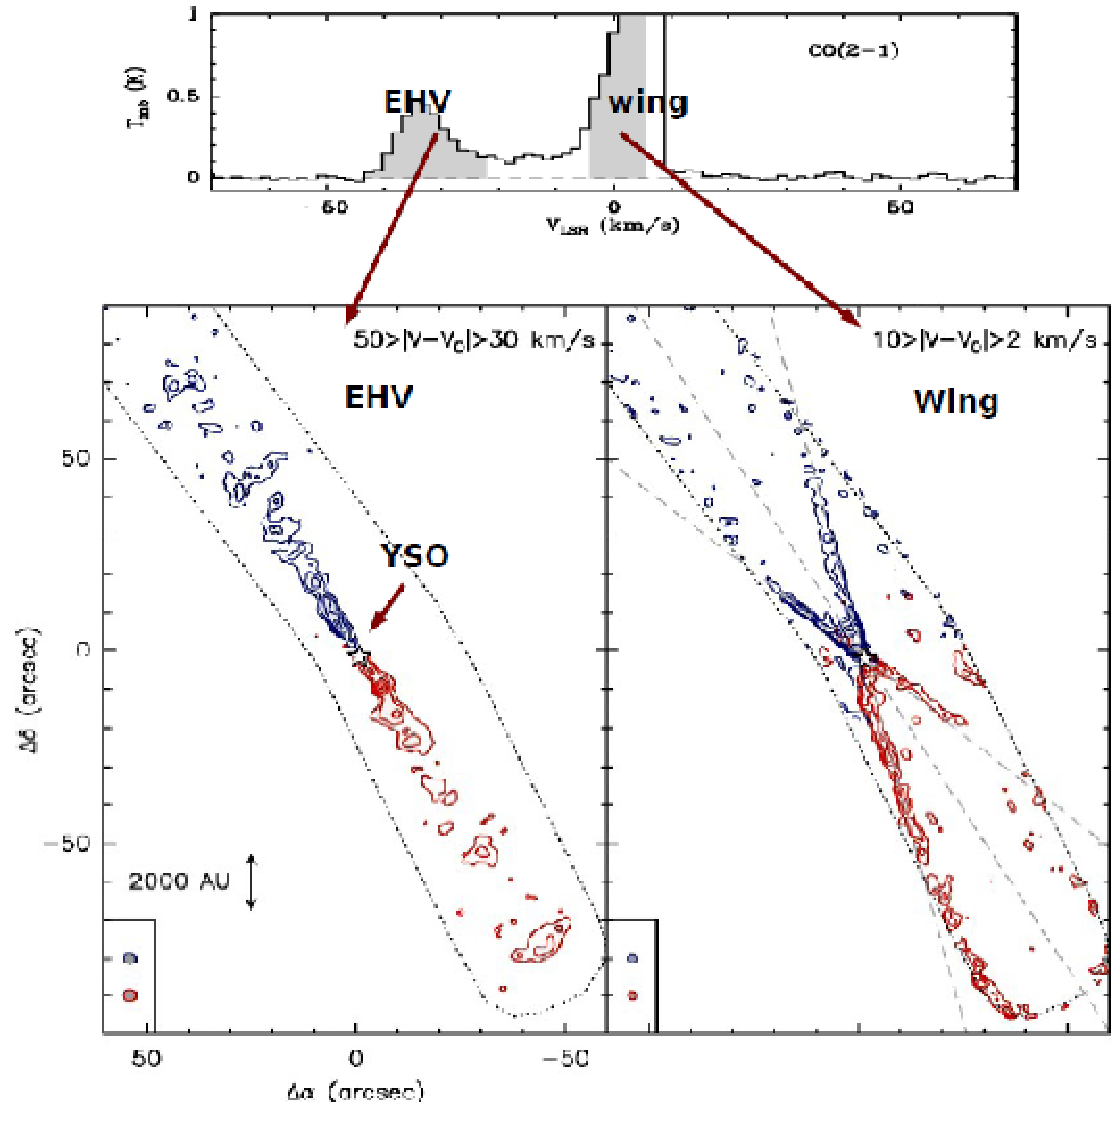
\includegraphics[height=4cm]{/Users/bhargavvaidya/MyProject/work/Leeds_Uni/SiOJets_New/PAPER/PFIGS/Tafalla2011.pdf}
\end{column}
\begin{column}{0.5\textwidth}
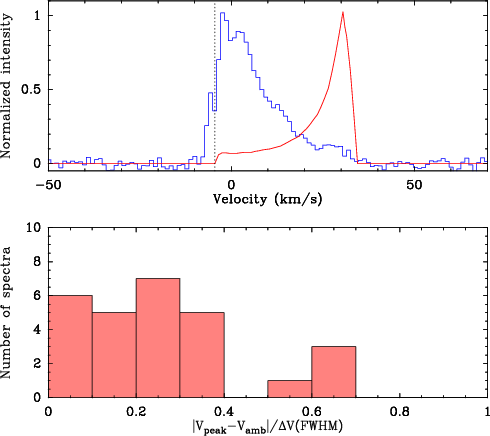
\includegraphics[height=4cm]{/Users/bhargavvaidya/MyProject/work/Leeds_Uni/SiOJets_New/PAPER/PFIGS/Tafalla2013.png}
\end{column}
\end{columns}
\end{frame}

\section{Numerical Approach}
\begin{frame}[t]
\frametitle{Methodology}
\begin{center}
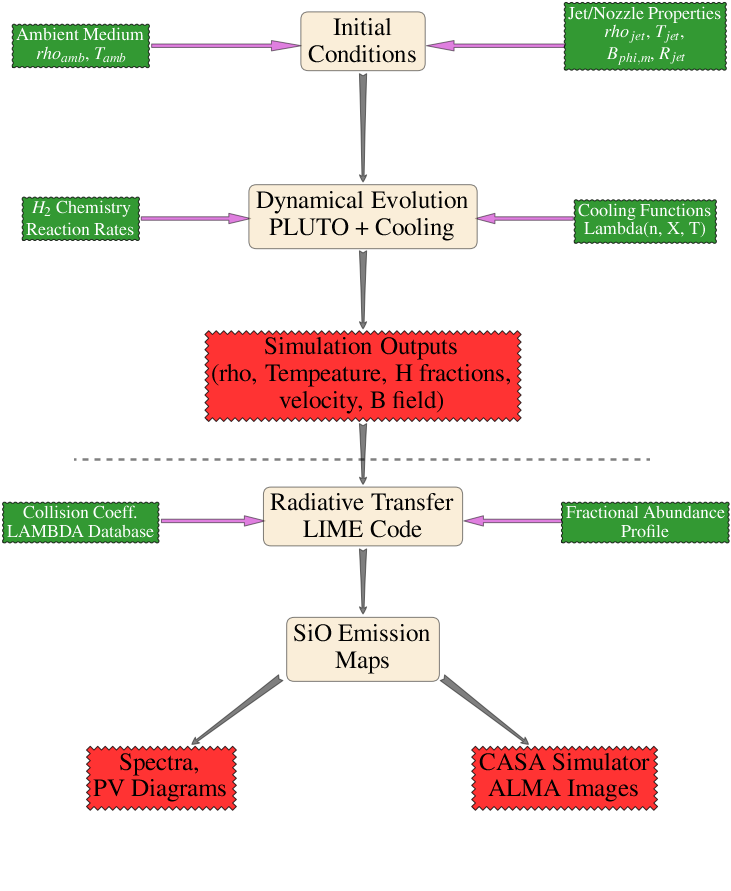
\includegraphics[height=7cm]{/Users/bhargavvaidya/MyProject/work/Leeds_Uni/SiOJets_New/PAPER/PFIGS/FlowChartJetProp.png}
\end{center}
\end{frame}


\begin{frame}
\frametitle{Initial Conditions}
\begin{columns}[T]
    \begin{column}{.4\textwidth}
     \begin{block}{Molecular Ambient Medium}
       Cold (T$_{\rm amb}$ $\sim$ 50\,K) \\ with decreasing density\\
       (\alert{Caselli, P., 2011})
       
    \end{block}
    \end{column}
    \begin{column}{.6\textwidth}  
      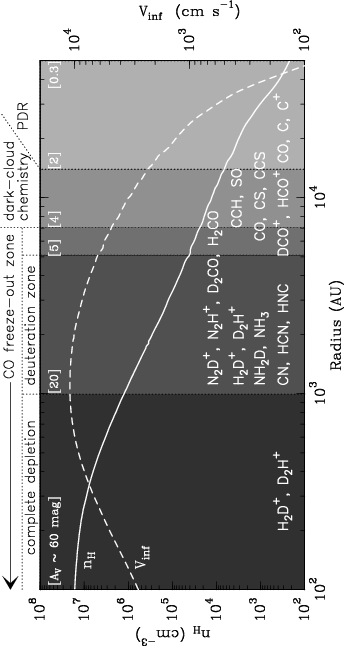
\includegraphics[width=3cm,height=6cm, angle=-90]{/Users/bhargavvaidya/MyProject/work/Leeds_Uni/SiOJets_New/PAPER/PFIGS/figure1_caselli.png}
    \end{column}
  \end{columns}
\vskip10pt 
\begin{columns}[T]
    \begin{column}{.4\textwidth}
     \begin{block}{Overdense MHD Jet}
       Propogating jet with \\ velocity perturbation \\
       $V_{\rm jet} = V_{\rm jet,0}[1 + sin(\frac{2\pi t}{70\, \rm
         yrs})]$\\
       (\alert{Stone\&Hardee, 2000})
    \end{block}
    \end{column}
    \begin{column}{.6\textwidth} 
      \hskip10pt
      \begin{tabular}{l l}
      \textbf{Quantity} & \textbf{Values}\\
      \hline\hline
      \smallskip
      $\eta$ & 2,3,10\\
      \smallskip
      $V_{\rm jet,0}$ & 100\, km\, s$^{-1}$\\
\smallskip
      Plasma $\beta_0$ & 10 $\sim$ 20$\mu$\,G \\
\smallskip
      $n_{\rm jet,0}$ & 10$^{5}$ cm$^{-3}$ \\
\smallskip
      $r_{\rm jet,0}$ & 160\,AU\\
\smallskip
      Composition & 1\% Ionic, 10\% Molecular,\\
      &89\% Atomic\\
      \hline
      \end{tabular}
    \end{column}
  \end{columns}


\end{frame}

\section{Cooling and Chemistry}
\begin{frame}
\frametitle{Cooling Prescriptions and H$_{2}$ Chemistry in PLUTO
 ( \alert{Mignone, 2007})}
\begin{columns}[C]
    \begin{column}{.5\textwidth}
     \begin{itemize}
     \item Adiabatic (No cooling)
     \item Power Law Cooling
     \item Atomic Cooling 
  \end{itemize}
    \end{column}
    \begin{column}{.5\textwidth} 
     \begin{itemize}
     \item Tabulated Cooling with {\em Fixed Initial Fractions}
     \item \textbf{Proper Molecular Cooling} (\alert{Vaidya et. al,
         \textit{in prep}, O'Sullivan's PhD Thesis})
     \end{itemize}

    \end{column}
  \end{columns}

\vskip10pt
\begin{columns}[C]
    \begin{column}{.5\textwidth}
      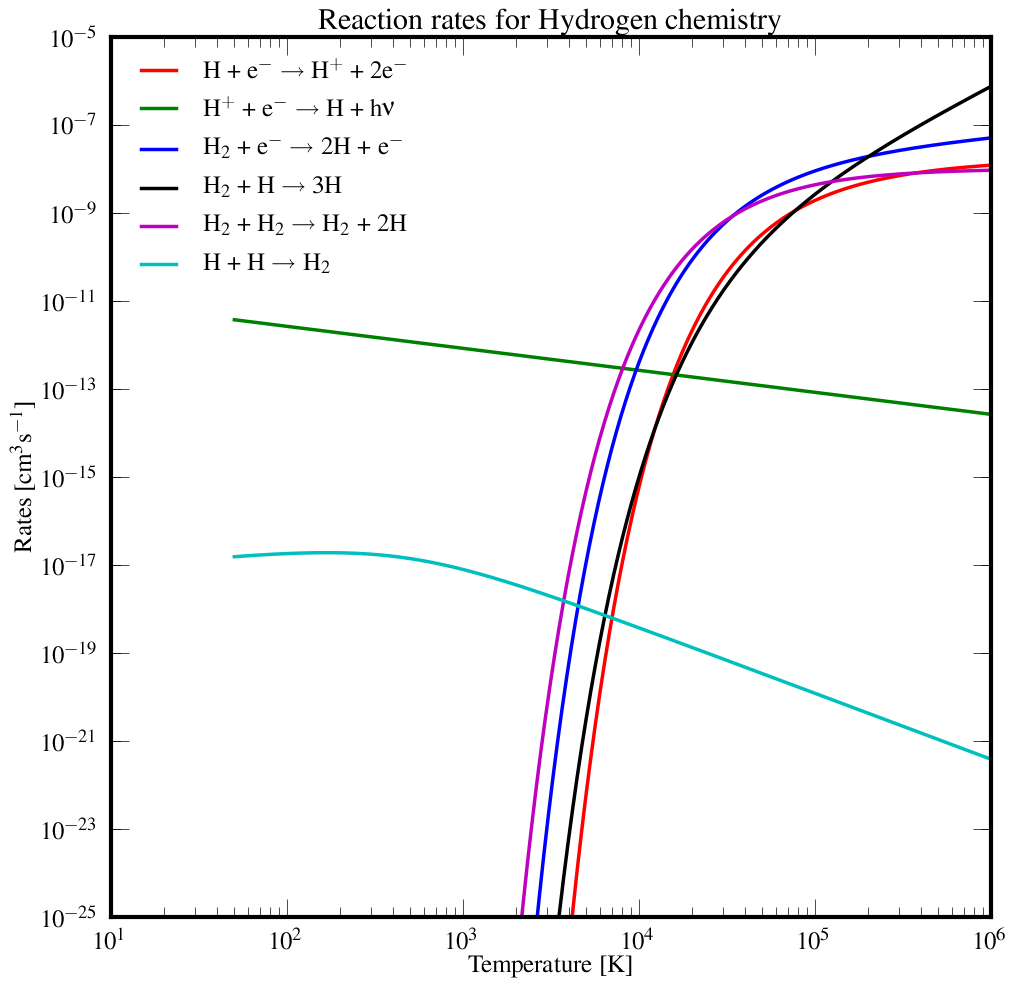
\includegraphics[width=5cm,height=5cm]{/Users/bhargavvaidya/MyProject/work/Leeds_Uni/SiOJets_New/PAPER/PFIGS/H2ReactionRates_paper.png}
    \end{column}
    \begin{column}{.5\textwidth}  
      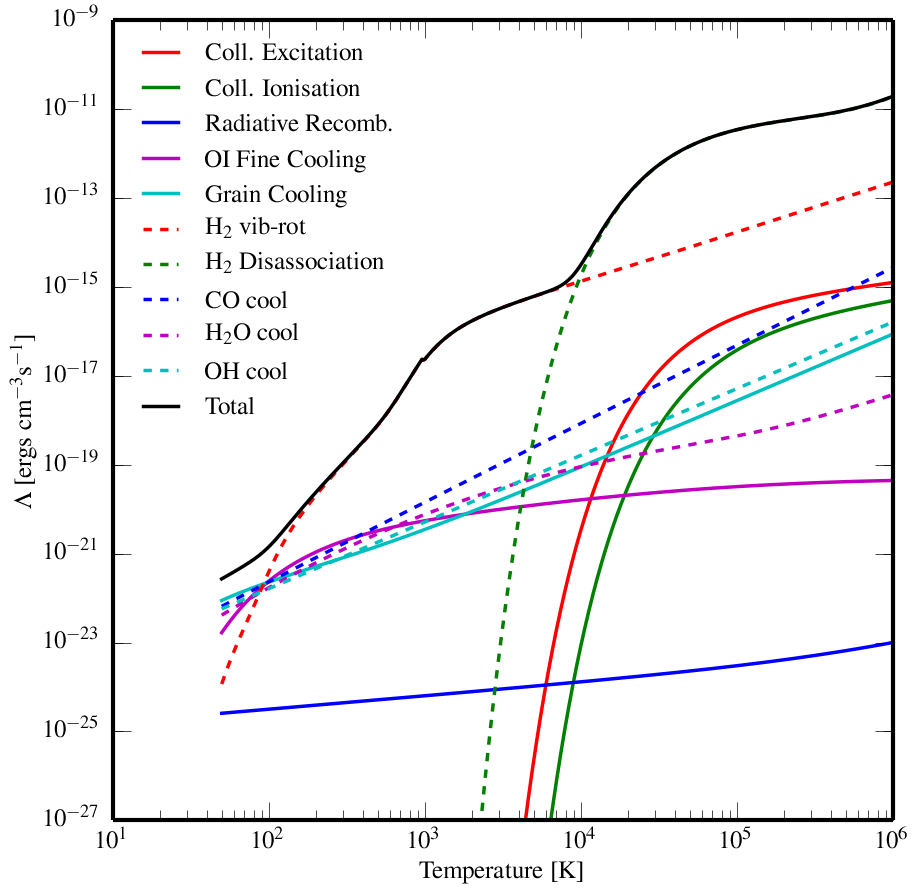
\includegraphics[width=5cm,height=5cm]{/Users/bhargavvaidya/MyProject/work/Leeds_Uni/SiOJets_New/PAPER/PFIGS/H2CoolingFuncs_full.png}
    \end{column}
  \end{columns}
\end{frame}


\begin{frame}[t]
\frametitle{Radiative Jet dynamics}
\begin{columns}[T]
    \begin{column}{.3\textwidth}
      \begin{block}{Impact of Cooling}
       \begin{itemize}
       \item $\eta$ = 10.0 \\
       \item Jet becomes thinner with more effective cooling \\
       \item Thermal Instabilities 
       \end{itemize}
       \end{block}
    \end{column}
    \begin{column}{.7\textwidth} 
     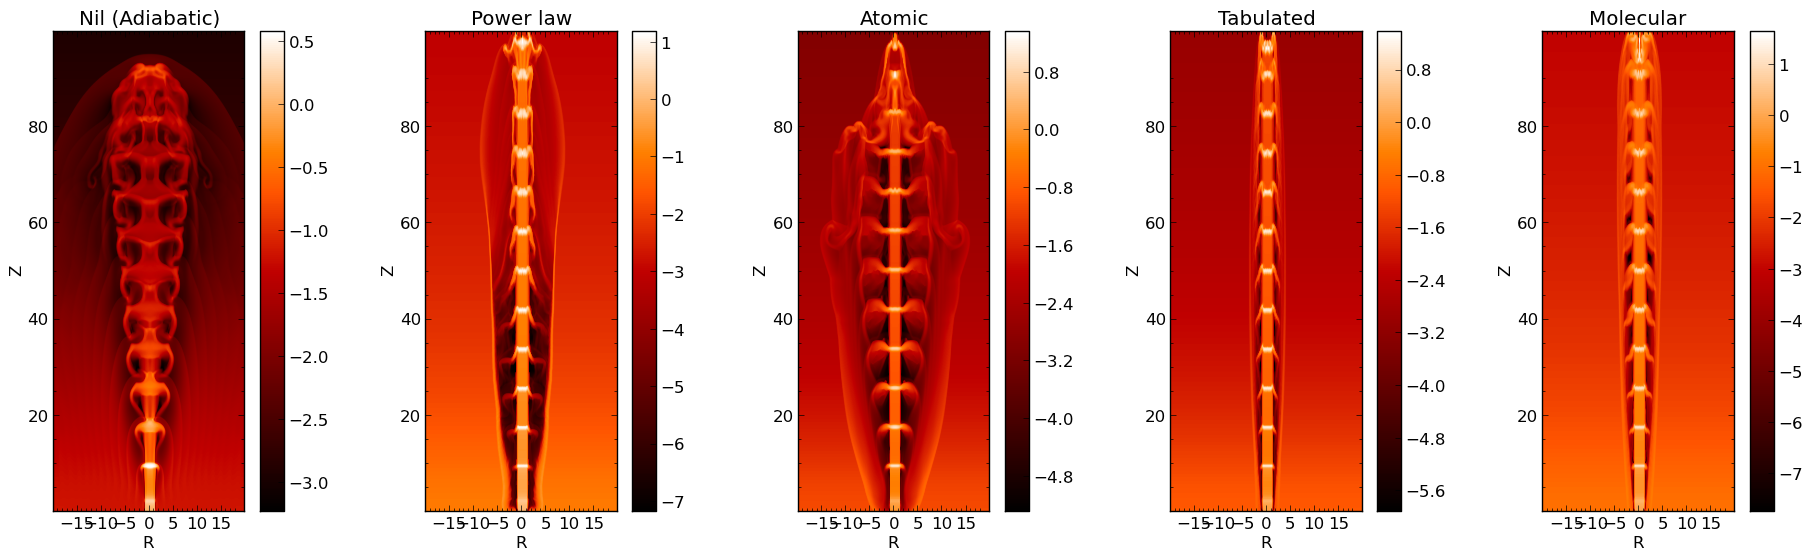
\includegraphics[width=8cm,height=3cm]{/Users/bhargavvaidya/MyProject/work/Leeds_Uni/SiOJets_New/PAPER/PFIGS/jetplt1_1010.png}
    \end{column}
  \end{columns}

\begin{columns}[T]
    \begin{column}{.3\textwidth}
       \begin{block}{Impact of Shocks}
      \begin{itemize}
      \item $\eta$ = 3.0 \\
      \item {\em Iternal Knots} - Formation and Destruction \\
      \item {\em Primary Bow shock} - Ionized Hydrogen with  T $>$ 20,000\,K.\\ 
      \end{itemize}
    \end{block}
    \end{column}
    \begin{column}{.7\textwidth} 
      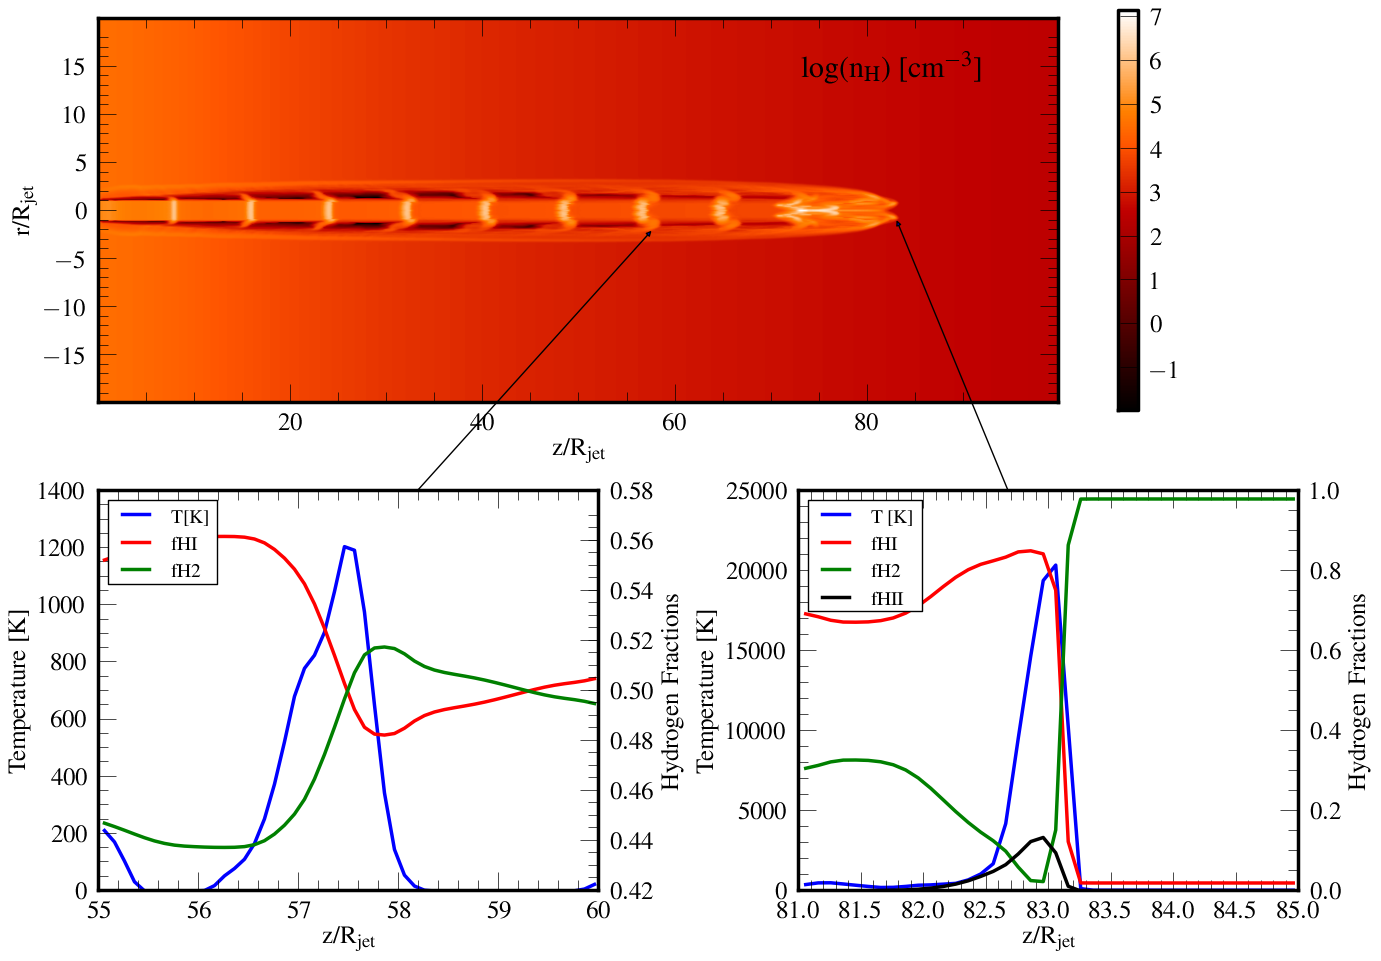
\includegraphics[width=6cm,height=4cm]{/Users/bhargavvaidya/MyProject/work/Leeds_Uni/SiOJets_New/PAPER/PFIGS/molcjet_310_molform.png}
   
    \end{column}
  \end{columns}
\end{frame}

\section[Rad. Transfer]{Radiative Transfer : Post-Processing}
\begin{frame}
\frametitle{Grid and Abundance}
\begin{columns}[T]
    \begin{column}{.4\textwidth}
      Line Modelling\\
      Engine [\textbf{LIME}] (\alert{Brinch \& Hogerheijde, 2010}) 
      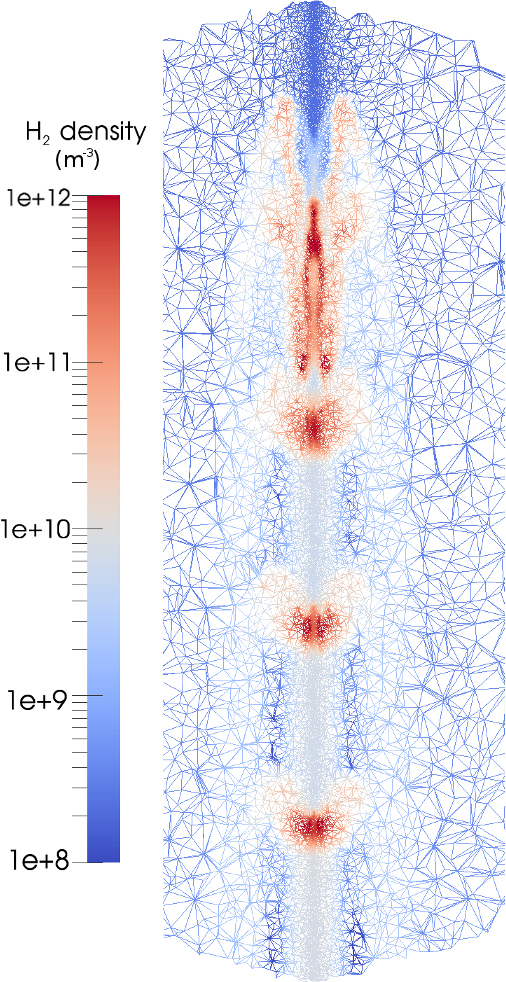
\includegraphics[width=3cm,height=6cm]{/Users/bhargavvaidya/MyProject/work/Leeds_Uni/SiOJets_New/PAPER/PFIGS/grid.png} 
    \end{column}
    \begin{column}{.6\textwidth}
      \small{
        \begin{itemize}
          \item n(SiO)/n(H2) as a function of shock velocity
           \item 10$^{-12}$ in Dark clouds (\alert{Ziurys, 1989}),\\
            10$^{-6}$ in fast outflows (\alert{Dutrey, 1997}).
          \item $\delta = V_{\rm shock}/ V_{\rm jet} = f(\eta) <= 1$
         \end{itemize}
       }
        
      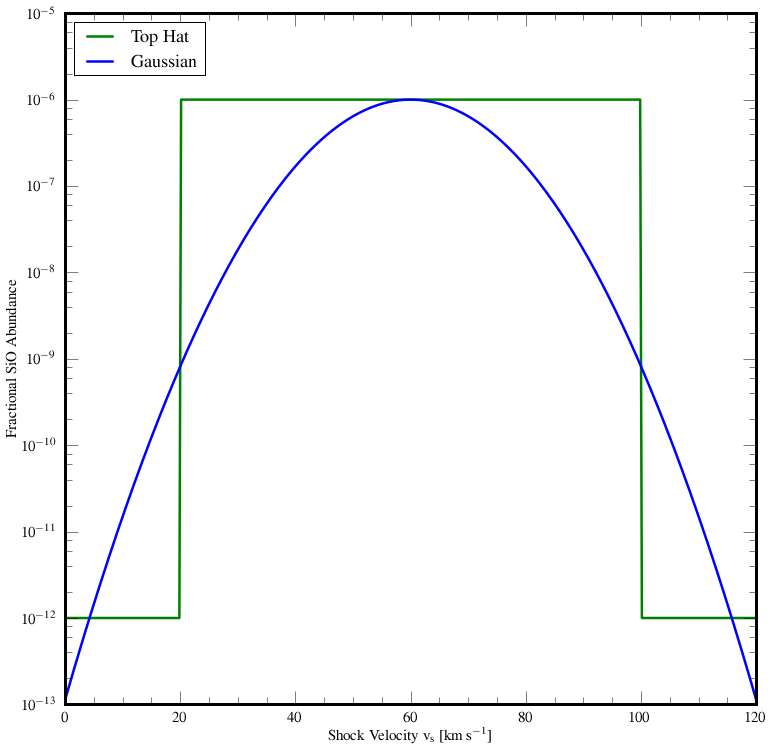
\includegraphics[width=5cm,height=5cm]{/Users/bhargavvaidya/MyProject/work/Leeds_Uni/SiOJets_New/PAPER/PFIGS/diffabunprof1.png}
      \end{column}
     \end{columns}   
\end{frame}

\begin{frame}[t]
\frametitle{Cooling and SiO Emission}
\tiny{
\begin{table}
\caption{Parameter runs with different cooling prescription and $\eta$ values}
\begin{tabular}{c | c | c | c | c | c | c }
\hline
Run & Cooling Mode & $\eta$ & \multicolumn{2}{|c|}{Top Hat Profile
  $\delta = 1$} & \multicolumn{2}{|c|}{Gaussian Profile $\delta =
  1$}\\
\hline\hline
&&& $\int T_{\rm MB}dV$ [K-km\,s$^{-1}$] & $\Delta$v [km s$^{-1}$] & $\int T_{\rm MB}dV$ [K-km\,s$^{-1}$] & $\Delta$v [km s$^{-1}$] \\
\hline
adi1010 & Nil (Adiabatic) & 10 & 2.91 & $>$40 & 0.25 & 40.0 \\
pow1010 & Power law & 10 & 0.64 & 8.0 & 0.02 & 10.0\\
atm1010 & Atomic & 10 & 2.04 & 36.0 & 0.58 & 38.0 \\
atm210 & Atomic & 2 & 3.21 & 18.0 & 0.64 & 20.0 \\
tab1010 & Tabulated & 10 & 0.75 & 11.0 & 0.09 & 10.0 \\
tab210 & Tabulated & 2 & 2.89 & 8.0 & 1.0 & 9.0 \\
mol1010 & Molecular & 10 & 1.10 & 10.0 & 0.1 & 11.0 \\
\color{red}{\textbf{mol310}} & Molecular & 3 & 3.3 & 14.0 & 0.66 & 12.0\\
\hline
\end{tabular}
\end{table}
}
\vskip10pt
\begin{columns}[T]

\begin{column}{0.3\textwidth}
  \begin{block}{Impact of Cooling}
    \begin{itemize}
      \item Jet flow with $\eta$ = 10 and $\beta$ = 10.0\\
      \item Integrated intensities with Gaussian Profile
        and $\delta < 1$.\\
      \item Convolved with a beam of FWHM = 2.5''
    \end{itemize}
  \end{block}
\end{column}

\begin{column}{0.7\textwidth}
 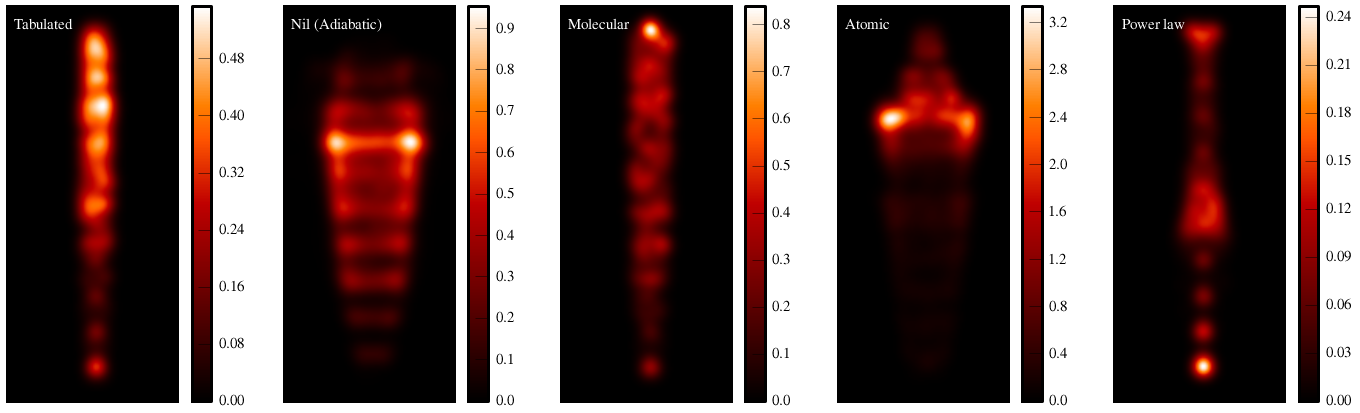
\includegraphics[width=8cm,height=3cm]{/Users/bhargavvaidya/MyProject/work/Leeds_Uni/SiOJets_New/PAPER/PFIGS/diffcool_EMgaussprof.png}
\end{column}
\end{columns}
\end{frame}

\section[Results]{Results : Line Emission, Spectra, PV Diagrams}
\begin{frame}[t]
\frametitle{SiO Multi-Line Movies}
\small{
\begin{itemize}
\item Molecular Jet with $\eta$ = 3.0, $\beta$ = 10.0 \\
\item Line Intensities with Gaussian Profile with $\delta < 1$. \\
\item Jet is in plane of sky and convolved with a beam of 2.5''
\end{itemize}
}
\begin{tabular}{ccc}
\textbf{J = 2-$>$1} & \textbf{J = 5-$>$ 4} & \textbf{J = 8-$>$ 7}\\
\animategraphics[width=3.5cm,height=5.5cm,autoplay]{5}{Img21/Img21_}{0000}{0010}
& 
\animategraphics[width=3.5cm,height=5.5cm,autoplay]{5}{Img54/Img54_}{0000}{0010}
&
\animategraphics[width=3.5cm,height=5.5cm,autoplay]{5}{Img87/Img87_}{0000}{0010}

\end{tabular}
\end{frame}

\begin{frame}
\frametitle{HH 211 - SiO Multi-Line Emission}
\begin{tabular}{ccc}
\textbf{J = 1-$>$0} (\alert{Chandler, 2001}) & \textbf{J = 5-$>$ 4}
(\alert{Hirano, 2006}) &
\textbf{J = 8-$>$ 7} (\alert{Palau, 2006})\\

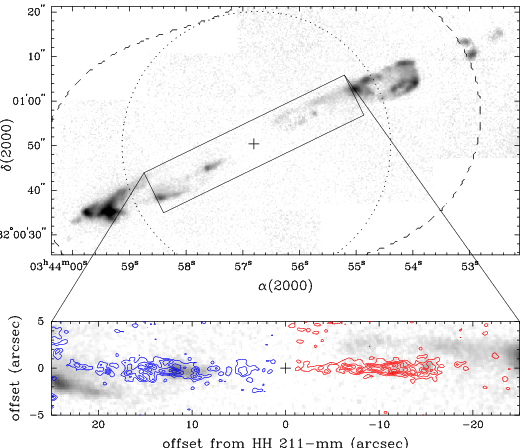
\includegraphics[width=3cm,height=3cm]{/Users/bhargavvaidya/MyProject/work/Leeds_Uni/SiOJets_New/PAPER/PFIGS/Chandler2001.png}
&
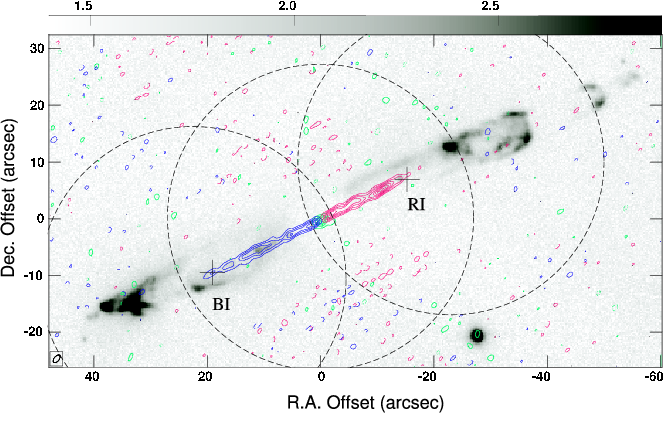
\includegraphics[width=3.5cm,height=2.5cm]{/Users/bhargavvaidya/MyProject/work/Leeds_Uni/SiOJets_New/PAPER/PFIGS/Hirano2005.png}
&
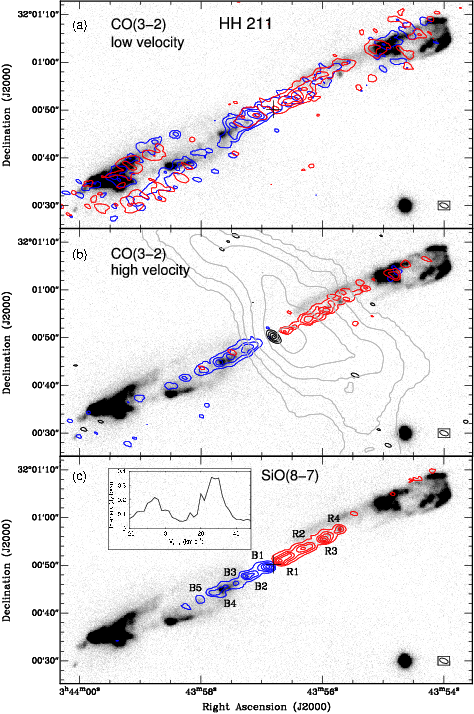
\includegraphics[width=2.5cm,height=3cm]{/Users/bhargavvaidya/MyProject/work/Leeds_Uni/SiOJets_New/PAPER/PFIGS/Palau2006.png}
\end{tabular}
\vskip10pt
\begin{columns}[T]
\begin{column}{0.3\textwidth}
 \begin{itemize}
    \item {\color{Brown}Low excitation} : Interaction of jet and medium.
    \item {\color{Brown}High excitation}: Internal knots.
 \end{itemize}
\end{column}

\begin{column}{0.7\textwidth}
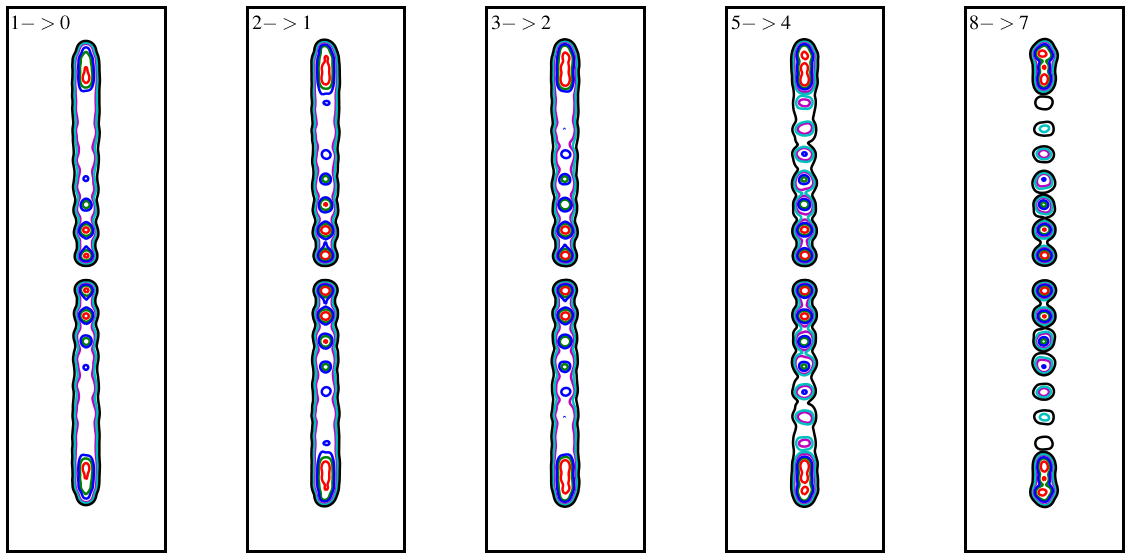
\includegraphics[width=7cm,height=3.5cm]{/Users/bhargavvaidya/MyProject/work/Leeds_Uni/SiOJets_New/PAPER/PFIGS/imshkvhcontomaps.png}
\end{column}
\end{columns} 
\end{frame}

\begin{frame}[c]
\frametitle{HH212 and L1448-mm : Spectra and Kinematics}
% \small{
% \begin{block}{Generic Features}
% \begin{itemize}
% \item L1448-mm : Weak line emission (T $\sim$ 0.3\,K) and peaks at 50
%   km\,s$^{-1}$ and a spectral width of about 20 km\,s$^{-1}$.\\
% \item SiO Multi-line analysis and LVG Modelling : Typical n(H$_{2}$)
%   $\sim$ 10$^{6}$ cm$^{-3}$ and Temperature of $>$ 500\,K.\\
% \item Line ratios from multi-line survey close to unity for both low
%   (HH212; ) and high mass (IRAS 17233-3606; ) young outflows. 
% \end{itemize}
% \end{block}
% }

\begin{columns}
 \begin{column}{0.33\textwidth}
Spectra (\alert{Codella, 1999})\\
 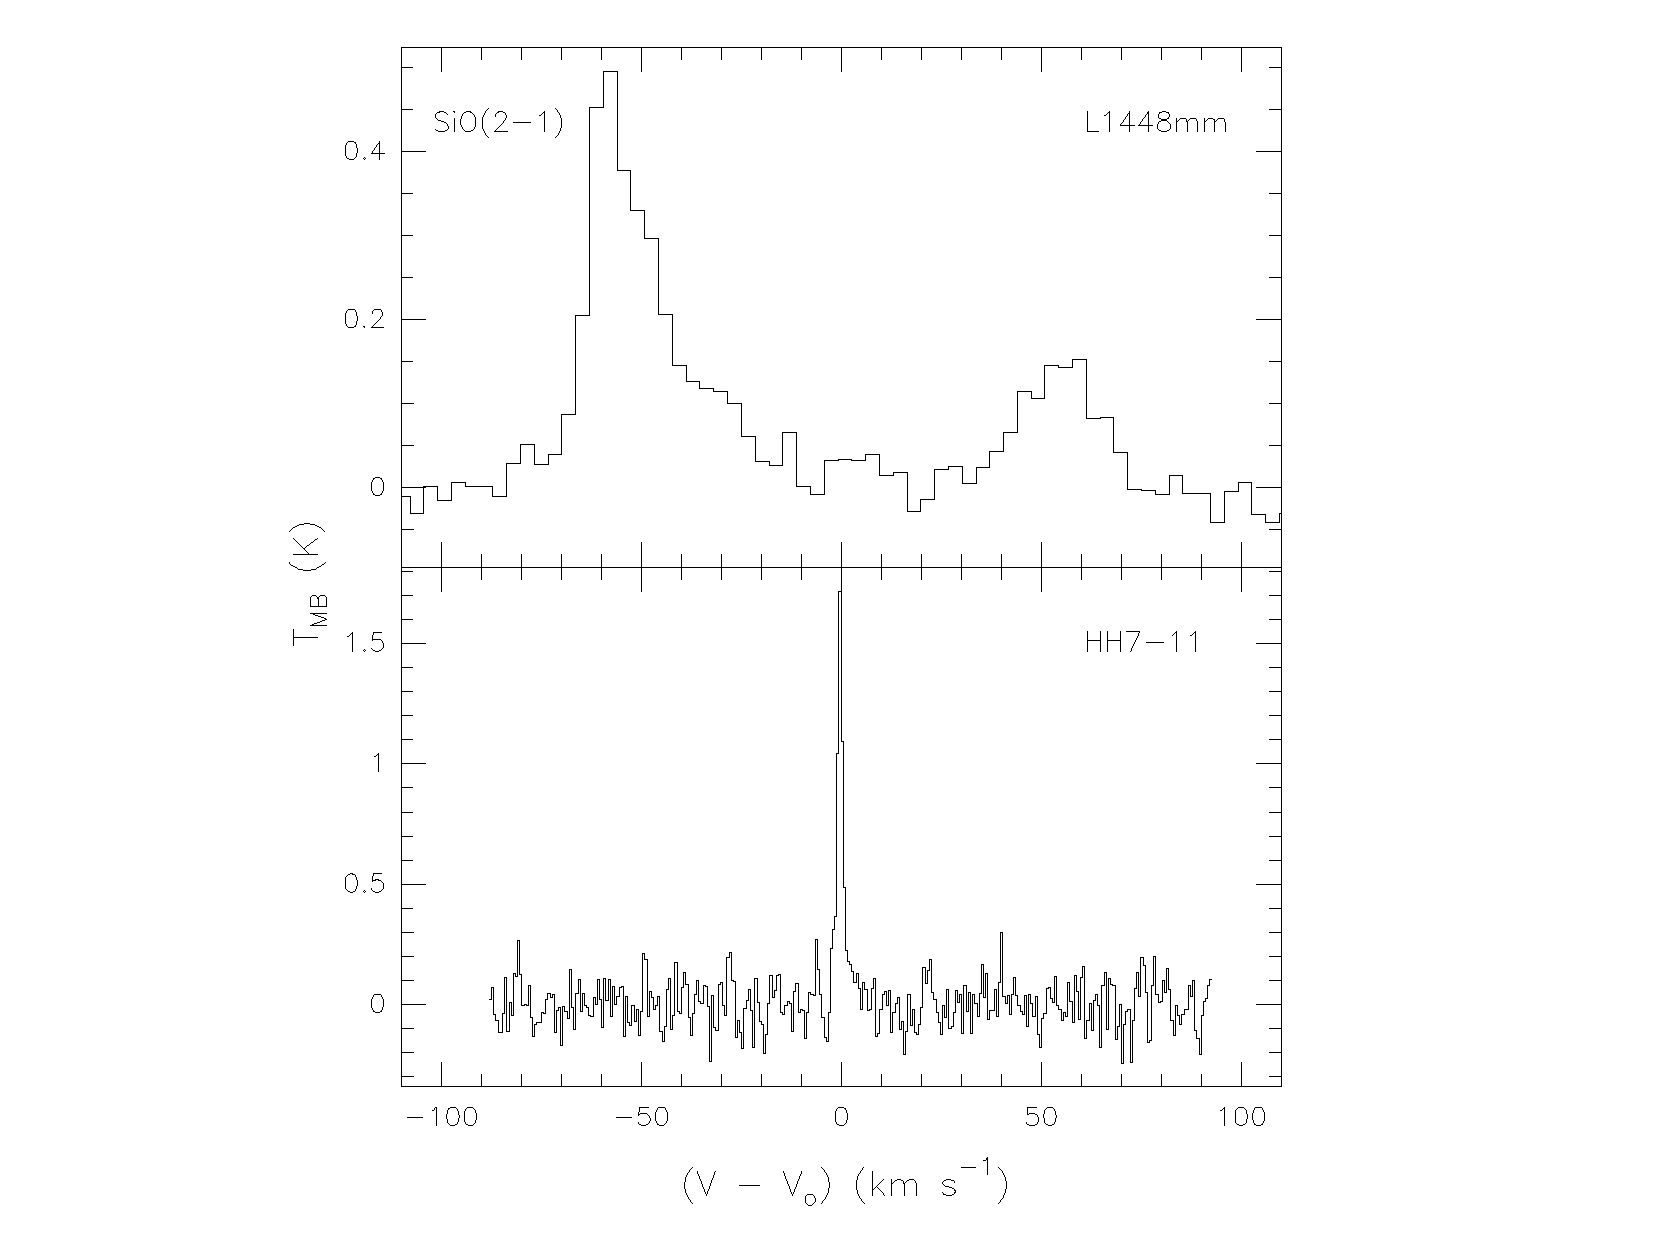
\includegraphics[width=4.0cm,height=4.0cm]{/Users/bhargavvaidya/MyProject/work/Leeds_Uni/SiOJets_New/PAPER/PFIGS/Codella1999.pdf}

 \end{column}

 \begin{column}{0.33\textwidth}
Line Ratios (\alert{Cabrit, 2007})\\
 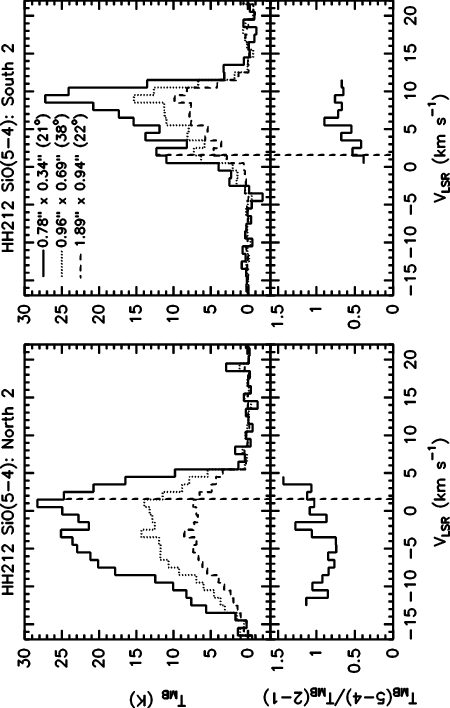
\includegraphics[width=3.0cm,height=4.0cm,angle=-90]{/Users/bhargavvaidya/MyProject/work/Leeds_Uni/SiOJets_New/PAPER/PFIGS/Cabrit2007.png}

 \end{column}

\begin{column}{0.33\textwidth}
Kinematics (\alert{Nisini, 2007})\\
 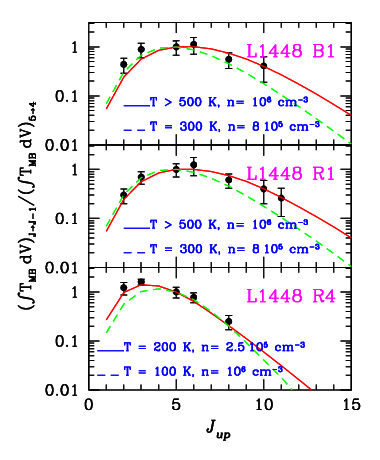
\includegraphics[width=3.5cm,height=4.0cm]{/Users/bhargavvaidya/MyProject/work/Leeds_Uni/SiOJets_New/PAPER/PFIGS/Nisini2007_2.png}\\

 \end{column}
 \end{columns}
\vskip10pt



 \end{frame}



\begin{frame}
\frametitle{Model Spectra and Line Ratios}
\begin{columns}[T]
\begin{column}{0.4\textwidth}
\begin{itemize}
\item Single dish spectra, Gaussian
  abundance profile, $\delta <$ 1, Inclination of 60$^{\circ}$. \\
\item High velocity emission consistent with generic observational features. \\
\item Missing Slow component ?
\item Optically Thick or Thin ?\\
\end{itemize}
\end{column}
\begin{column}{0.6\textwidth}
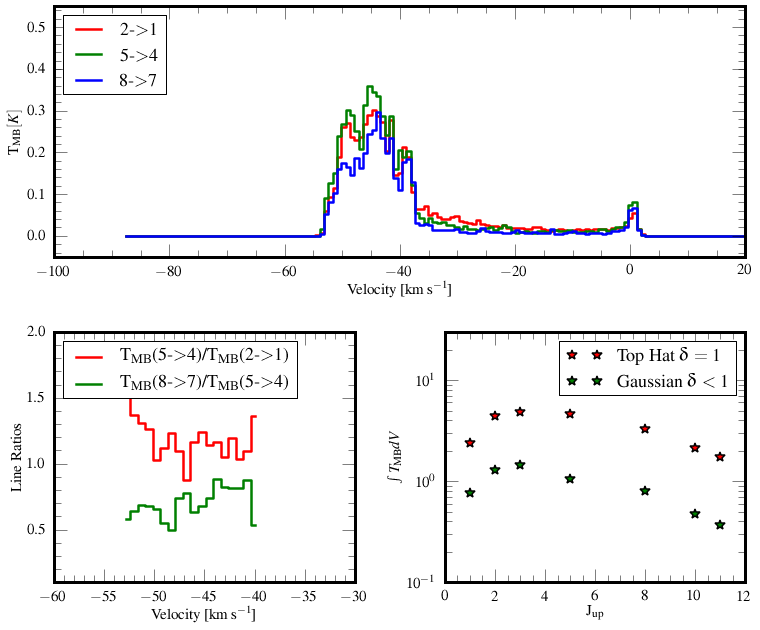
\includegraphics[width=6cm,height=6cm]{/Users/bhargavvaidya/MyProject/work/Leeds_Uni/SiOJets_New/PAPER/PFIGS/LineRatio_THDeq1.png}
\end{column}
\end{columns}
\end{frame}

\begin{frame}
\frametitle{PV Diagrams}
\begin{columns}[T]
\begin{column}{0.5\textwidth}
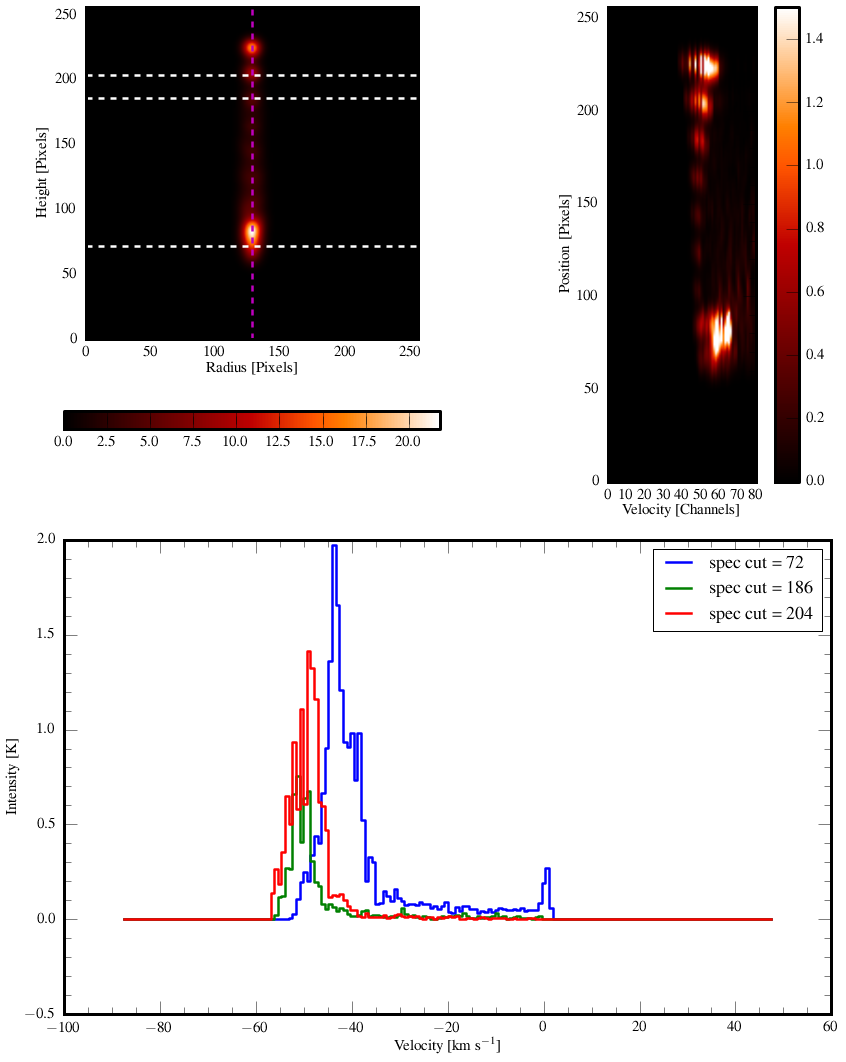
\includegraphics[width=5cm,height=7cm]{/Users/bhargavvaidya/MyProject/work/Leeds_Uni/SiOJets_New/PAPER/PFIGS/refrun_21_60_emspecpv.png}
\end{column}
\begin{column}{0.5\textwidth}
IRAS 04166+2706 (\alert{Santiago-Garcia, 2009}). 
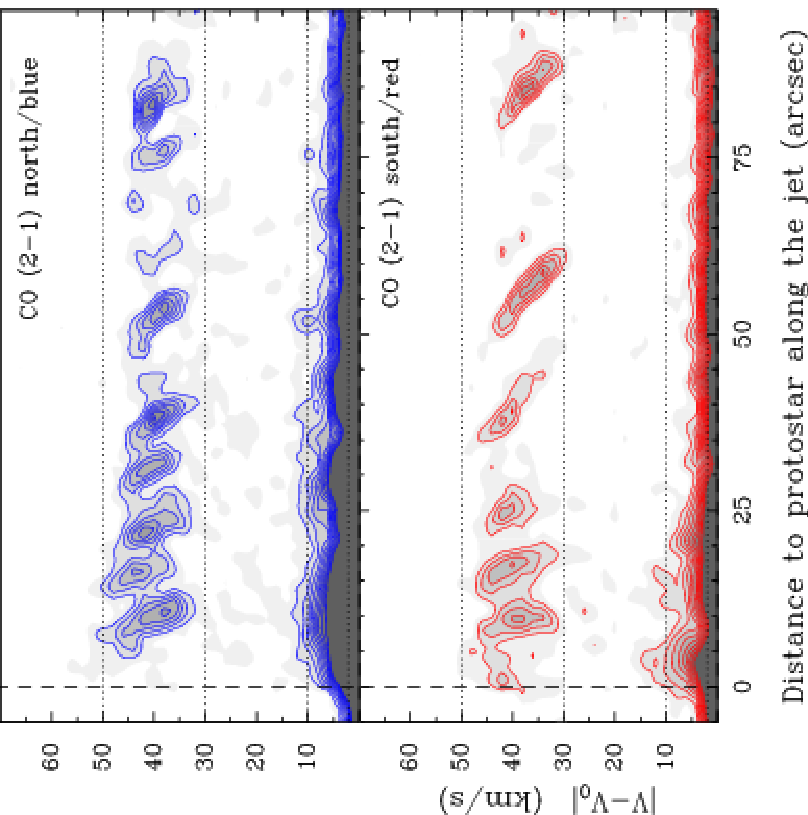
\includegraphics[width=5cm,height=5cm,angle=-180]{/Users/bhargavvaidya/MyProject/work/Leeds_Uni/SiOJets_New/PAPER/PFIGS/Santiago2009.pdf}
\end{column}
\end{columns}

\end{frame}

\begin{frame}[c]
\frametitle{Effects of Abundance}
\begin{columns}[c]
\begin{column}{0.9\textwidth}
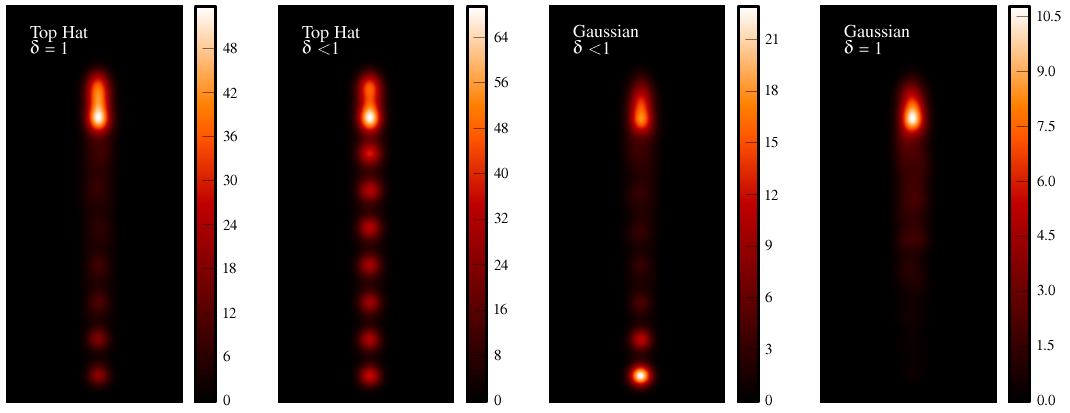
\includegraphics[width=9cm,height=3cm]{/Users/bhargavvaidya/MyProject/work/Leeds_Uni/SiOJets_New/PAPER/PFIGS/EM_gaussandth.png}
\end{column}
\end{columns}
\vskip10pt
\begin{columns}[c]
\begin{column}{0.9\textwidth}
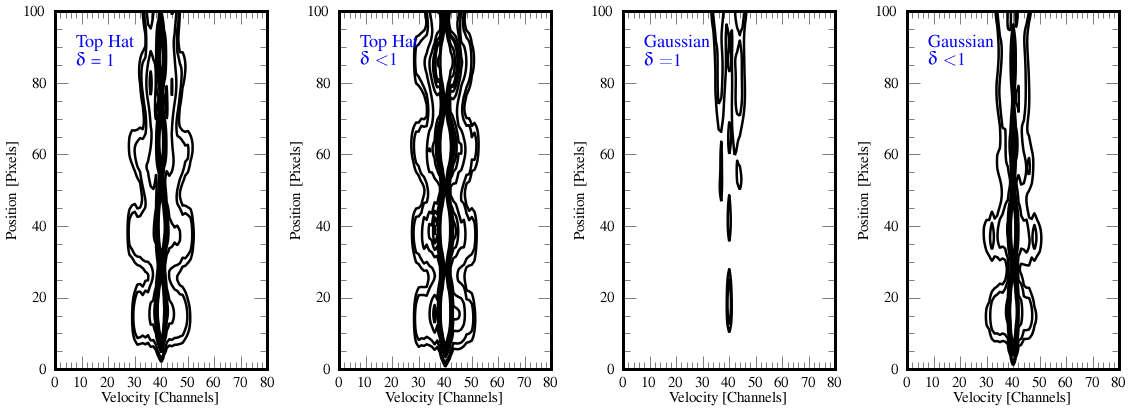
\includegraphics[width=9cm,height=3cm]{/Users/bhargavvaidya/MyProject/work/Leeds_Uni/SiOJets_New/PAPER/PFIGS/PV_gaussandth.png}
\end{column}
\end{columns}

\end{frame}

\section{Summary}
\begin{frame}
\frametitle{Summary}
\begin{itemize}
\item Axi-symmetric MHD Jet propagation simulations with
  \alert{Molecular cooling and Hydrogen chemistry} for the context of studying molecular outflows in Class 0 phase.

\item Extremely High Velocity(EHV) emission of SiO seen in some young
  outflows are produced by \alert{interaction of internal knots with ambient
  medium via J-shocks}

\item Our model can very \alert{reproduce observational features} like :
  \begin{itemize}
    \item Integrated intensity of EHV emission.
    \item Spectral shape and line ratios seen in SiO emission from some of these Class 0 Outflows.
    \item Knotty features of PV diagrams. 
  \end{itemize}

\item \alert{Outlook}
\begin{itemize}
  \item Longer, 3D, AMR simulations which consistently produce
    internal knots (\alert{Gomez et. al 2013}).
  \item Consistent modeling for dust chemistry to have better
    constraints on SiO abundance.
  \item Slower wider component seen in chemical molecules like CO, H$_{2}$O (Herschel WISH
    Survey, \alert{Tafalla et. al., 2013}).
\end{itemize}

\item \alert{ALMA Maps !}
\end{itemize}
\end{frame}

\begin{frame}[t]
\frametitle{ALMA Maps}
\begin{columns}[T]
\begin{column}{0.3\textwidth}
\begin{block}{CASA Simulation}
\begin{itemize}
\item Source Distance : 300 pc 
\item Cycle 1 --  Bands(Beam Size) :  3(0.72''), 6(0.47'') and 7(0.58'') 
\item Integration time : 30 min
\item Velocity Resolution : 1 km s$^{-1}$
\end{itemize}
\end{block}
\end{column}
\begin{column}{0.7\textwidth}
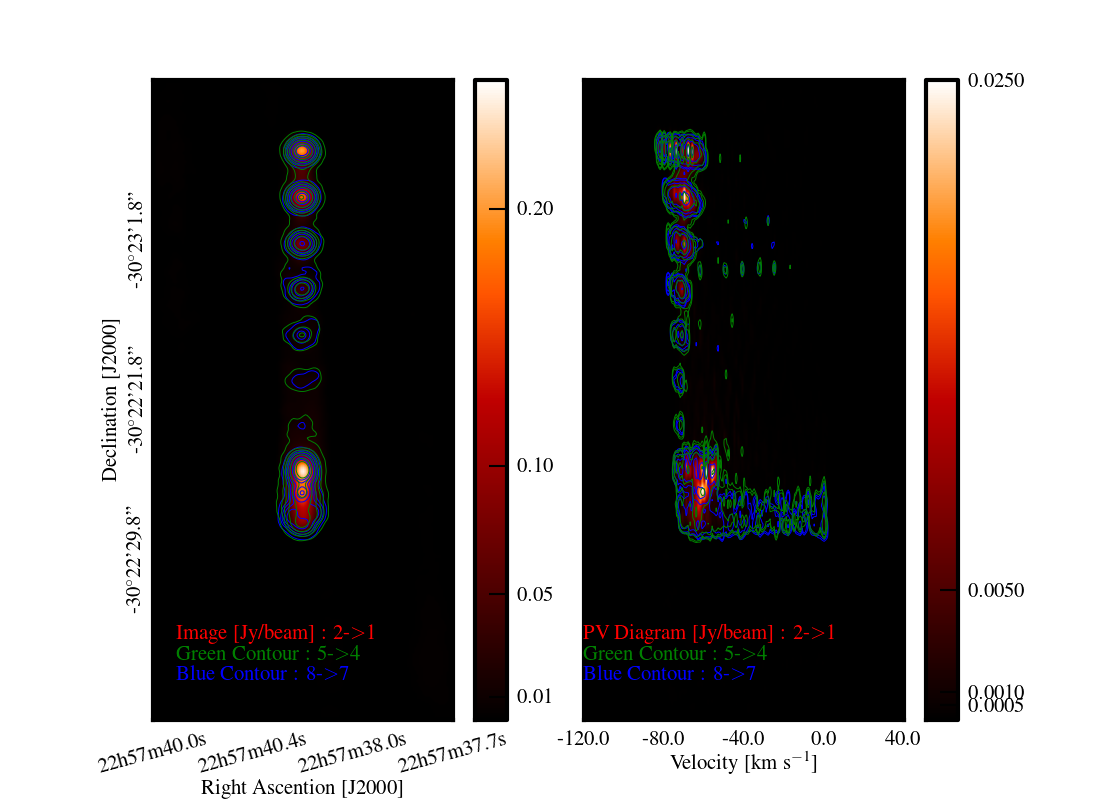
\includegraphics[width=8.5cm]{/Users/bhargavvaidya/MyProject/work/Leeds_Uni/SiOJets_New/PAPER/PFIGS/ALMAmaps3.png}
\end{column}
\end{columns}
\end{frame}

\end{document}

